\section{问题三：日内光伏预报与合同调整}

\subsection{官方预报的因果处理}

附件给出0、6、12、18时发布的逐小时光伏预报。对发布时刻 $h\in\{0,6,12,18\}$，先将未来整点预报裁剪为非负，再以当前时刻已经观测的光伏端点为锚，线性插值到10分钟网格。1月1日0时没有前一已观测端点，锚值取0。这样既避免光伏出现负值，也防止插值曲线在更新时刻与真实已观测前缀脱节。

令 $F_{d,h,\ell}$ 为日$d$在时刻$h$对提前 $\ell$ 小时目标的官方预报，真实值为 $V_{d,h+\ell}$。偏差样本定义为
\begin{equation}
 r_{d,h,\ell}=V_{d,h+\ell}-F_{d,h,\ell}.
 \label{eq:official-residual}
\end{equation}
在日期$d$进行修正时，只取最近60个已完成日期的同一发布时刻残差均值，不能使用当天尚未完成的残差。经非负裁剪的修正预报为
\begin{equation}
 \widehat V^{\mathrm{off}}_{d,h,\ell}
 =\max\left\{0,F_{d,h,\ell}+\frac{1}{|\mathcal R_{d,h}|}
 \sum_{k\in\mathcal R_{d,h}}r_{k,h,\ell}\right\}.
 \label{eq:bias-correction}
\end{equation}
若历史为空，则修正量为0。

图\ref{fig:q3-error}给出原始预报误差随发布时间和提前期的变化。对相同的当日剩余目标，0、6、12、18时原始MAE分别为186.7347、129.0903、35.1985和0.00036 kW，修正后分别为188.1883、130.9920、35.5854和0.00051 kW。修正降低了平均偏差的绝对值，但MAE并未改善；18时剩余目标主要处于夜间，满足真实光伏大于100 kW的MAPE有效样本数为0，故不报告MAPE数值。该结果说明“消除均值偏差”不等同于“降低绝对误差”。

\begin{figure}[H]
  \centering
  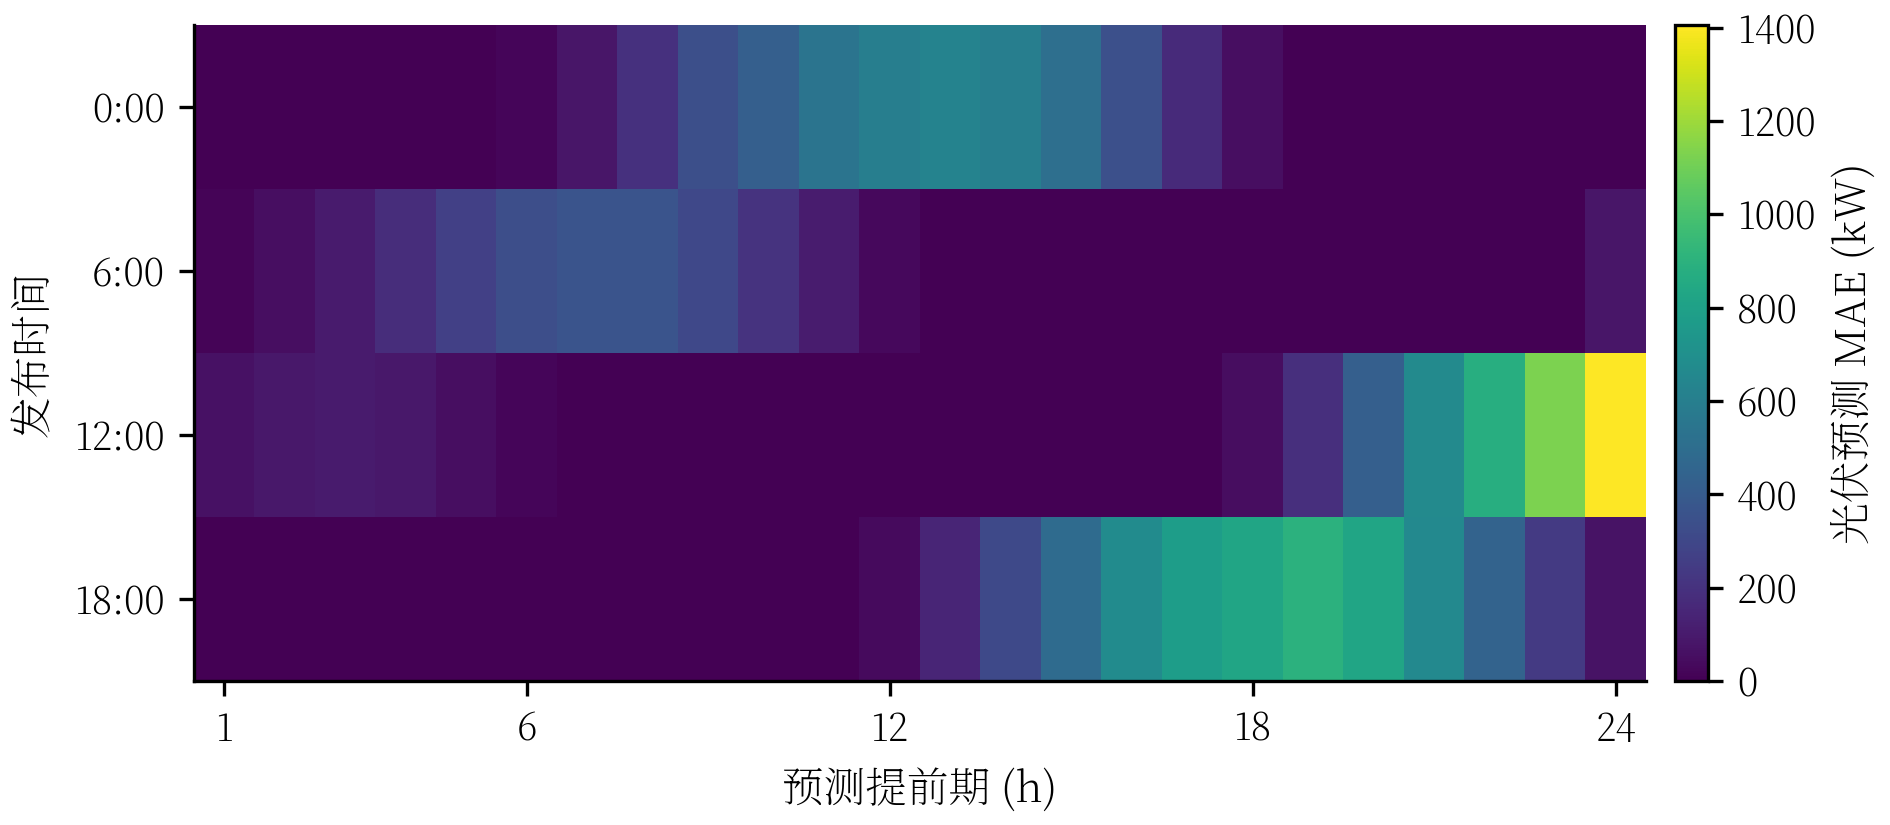
\includegraphics[width=0.98\textwidth]{figs/raw_q3_forecast_error.png}
  \caption{官方光伏预报MAE随发布时刻与提前期的变化。跨年不可得目标被排除，颜色不代表概率置信度。}
  \label{fig:q3-raw}
  \label{fig:q3-error}
\end{figure}

\subsection{滚动合同与结算模型}

0时先生成全天合同 $p_t$。每次更新到达后，对 $t\ge 6h$、$12h$ 或 $18h$ 的尚未执行时槽重新求解，已执行合同和实际能量流保持不变。规划中的负荷预测仍来自相似日模型；安全光伏轨迹用更新后的官方预报替代点预测，并继续使用过去残差形成保守余量。当天SOC从前一事件末端传递到下一事件，不因重规划而重置。

设 $q_t$ 为某时槽最后一次更新后真正执行的合同。主结算解释以0时合同 $p_t$ 为不可变基准，并按最终合同只结算一次：
\begin{equation}
 C_t=c_t\left[\min(p_t,q_t)+1.5\pos{q_t-p_t}
 +0.5\pos{p_t-q_t}\right]+5c_tu_t .
 \label{eq:settlement-primary}
\end{equation}
其中下调合同对应半价退还的净效果；多次中间修改不逐次重复收费。为检验题意解释的影响，再对同一物理执行轨迹计算
\begin{equation}
 C_t^{\mathrm{alt}}=c_t\left[p_t+1.5\pos{q_t-p_t}
 +0.5\pos{p_t-q_t}\right]+5c_tu_t .
 \label{eq:settlement-alt}
\end{equation}
式\eqref{eq:settlement-alt}把下调量作为额外费用而非退款。它只用于同策略重新计费，没有在该规则下重新优化；在允许合同闲置且无退款收益的情况下，下调动作甚至可能被不下调严格支配。因此，两种费用必须分别解释，不能混称为同一个最优问题。

以 $p_t=10$ kWh、$c_t=1$ 元/kWh且无应急购电为例，最终合同 $q_t=5,10,15$ kWh时，主结算费用分别为7.5、10和17.5元；替代结算分别为12.5、10和17.5元。该例说明两式只在下调区间不同：主式把未执行的5 kWh基准合同按半价净退款处理，替代式则在原合同上再加半价下调费用。若不先明确这一差别，同一合同轨迹会得到不同的频率建议。

滚动求解还必须保持事件间状态一致。设相邻更新时刻为 $h_j<h_{j+1}$，在 $h_j$ 只求解尚未执行的剩余段；区间 $[h_j,h_{j+1})$ 按真实值执行后，得到的SOC是下一次LP的固定初态。已执行合同、充放电和应急量均不回写。因而最终日费用可以按144个槽各自的最后有效合同相加，而不能把四次规划目标相加。

图\ref{fig:q3-update}展示6月21日合同随预报更新发生有方向的改变。图中的实际净负荷尚未扣除储能动作，因此不能把合同曲线与净负荷曲线的差直接解释为应急量或弃光量。

\begin{figure}[H]
  \centering
  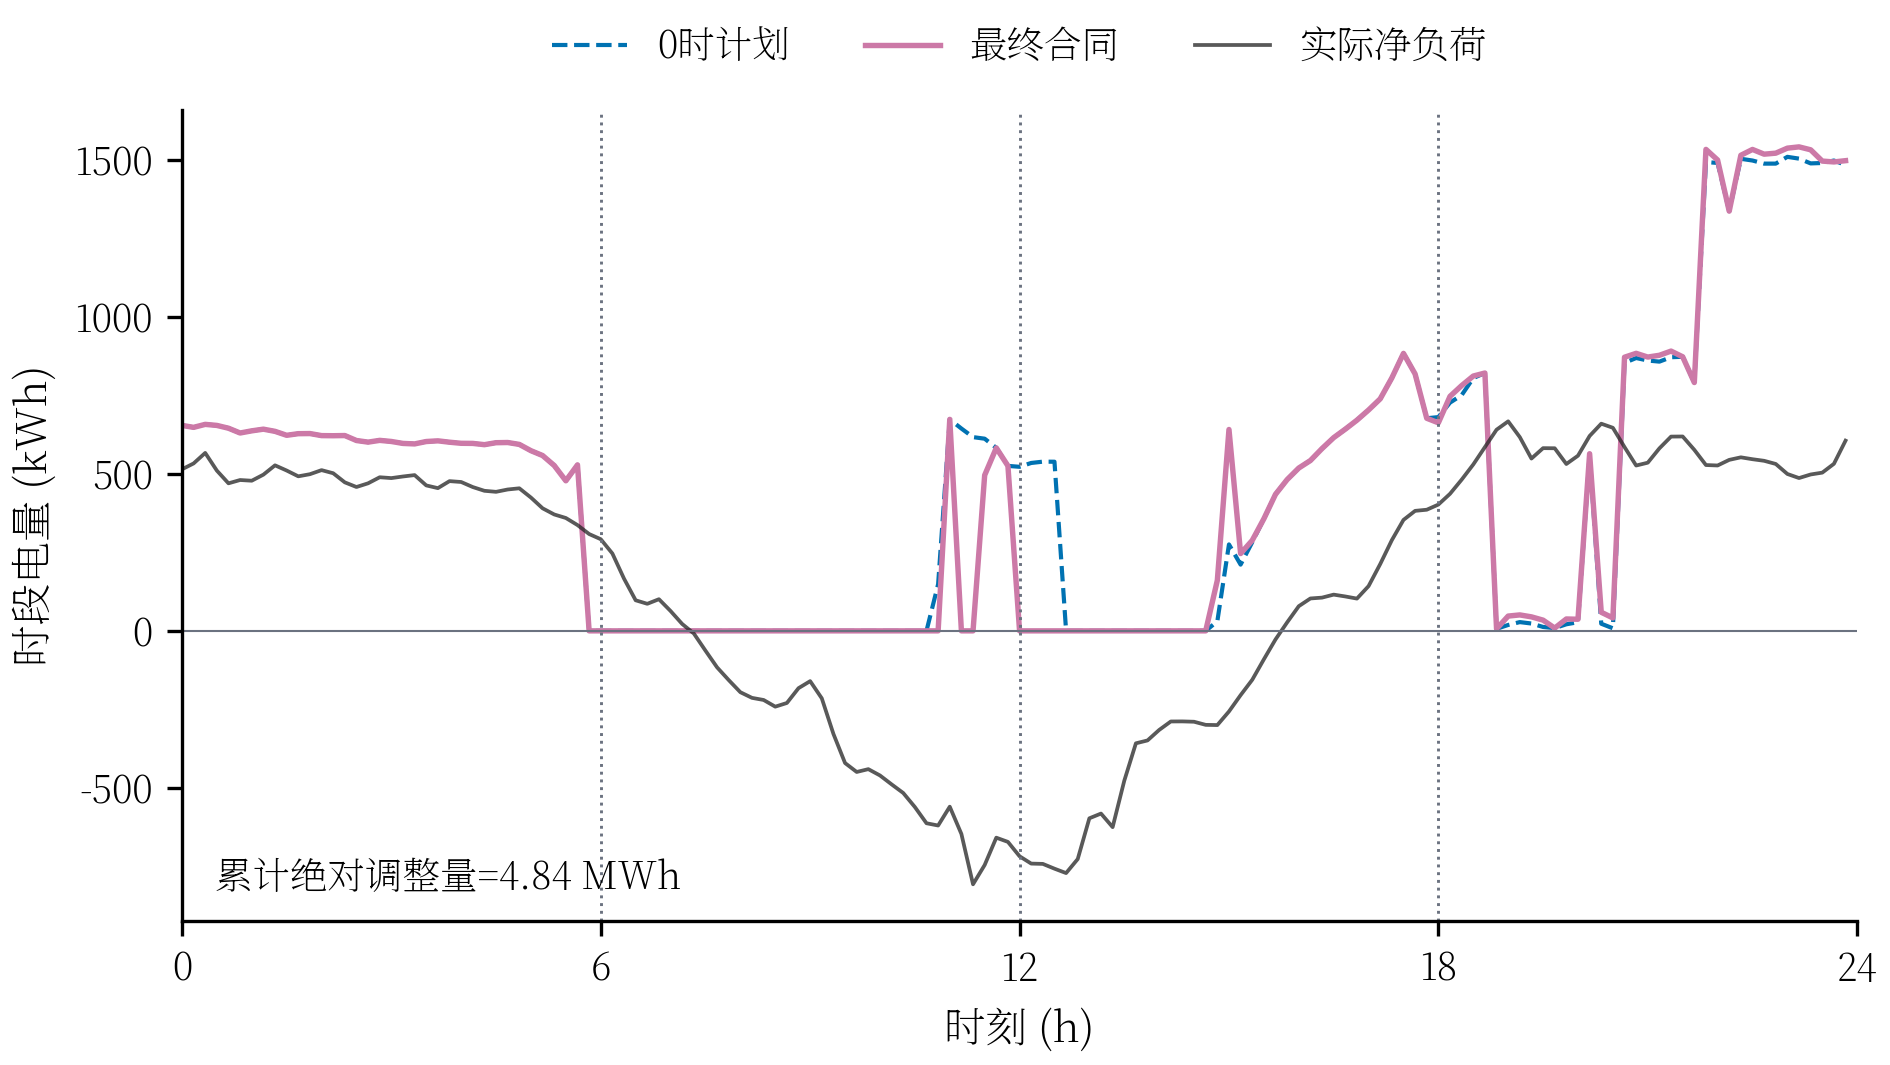
\includegraphics[width=0.97\textwidth]{figs/process_q3_contract_updates.png}
  \caption{6月21日0时初始合同与日内最终合同。竖线为6、12、18时更新事件。}
  \label{fig:q3-update}
\end{figure}

\subsection{主策略结果}

问题三334日现金费用为 $16279696.6905$ 元，应急购电量为 $115458.1457\,\mathrm{kWh}$，闲置合同为 $3093394.8432\,\mathrm{kWh}$，弃光为 $1841583.5122\,\mathrm{kWh}$，年末SOC为 $10649.4342\,\mathrm{kWh}$。相对问题二，现金费用减少 $2484469.2430$ 元，应急购电减少约80.03\%。但这项差异同时改变了光伏信息来源和合同更新规则，并非“只增加更新次数”的纯频率效应。

四个代表日中，3月20日、6月21日和9月23日费用下降，而12月21日费用由 $63120.3057$ 元上升为 $65731.5948$ 元，应急购电也从 $382.2268$ 增至 $979.7444\,\mathrm{kWh}$。因此，年度改善不能被写成逐日占优。详细代表日购电、储能与应急结果见附录\ref{app:tables}。

\subsection{相同0时信息下的更新频率分析}

为尽量分离“0时信息不同”的影响，固定0时采用问题三的同一官方信息，比较只在0时、0/12时、0/6/12/18时和每2小时更新四组方案。2小时情形并非附件提供的新官方预报：在非官方发布时刻，模型沿用最近一次已发布预报，并以当天已经实现的最多18个10分钟槽偏差构造3小时指数衰减的合成短临更新；该更新只调整安全光伏，同时保持安全负荷轨迹，不重新标定场景概率。

\noindent 四组费用及两种结算的对照列于表\ref{tab:q3freq}。负的“相对6小时节约”表示候选方案更贵，而不是负费用。

\begin{table}[H]
\centering
\caption{固定电价下相同0时信息的更新集合比较}
\label{tab:q3freq}
\resizebox{\textwidth}{!}{%
\begin{tabular}{lrrr}
\toprule
更新集合 & 主结算费用/元 & 相对6小时节约/元 & 替代结算相对6小时节约/元\\
\midrule
仅0时 & 17,613,329.64 & $-1,333,632.95$ & $-537,280.34$\\
0、12时 & 17,143,902.65 & $-864,205.96$ & $-659,112.90$\\
每6小时 & 16,279,696.69 & 0 & 0\\
每2小时合成更新 & 15,571,353.39 & 708,343.30 & 127,065.26\\
\bottomrule
\end{tabular}}
\end{table}

2小时方案在主结算下相对6小时方案节约4.3511\%，全年增加2672次更新。若每次额外更新的综合通信、计算和运维成本记为$k$，则其净收益为
\begin{equation}
 B_{2h}=708343.3002-2672k.
 \label{eq:breakeven-fixed}
\end{equation}
故盈亏平衡阈值为 $k^*=265.0985$ 元/次。四个代表日在主结算口径下均不劣，但替代结算下总节约仅约12.71万元，且仅0时与12小时方案的排序会反转。图\ref{fig:q3-frequency}直观显示结算解释对更新价值的影响，因此合理建议是“在主结算成立且每次增量成本低于阈值时采用2小时合成更新”，而不是无条件追求最高更新频率。

\begin{figure}[H]
  \centering
  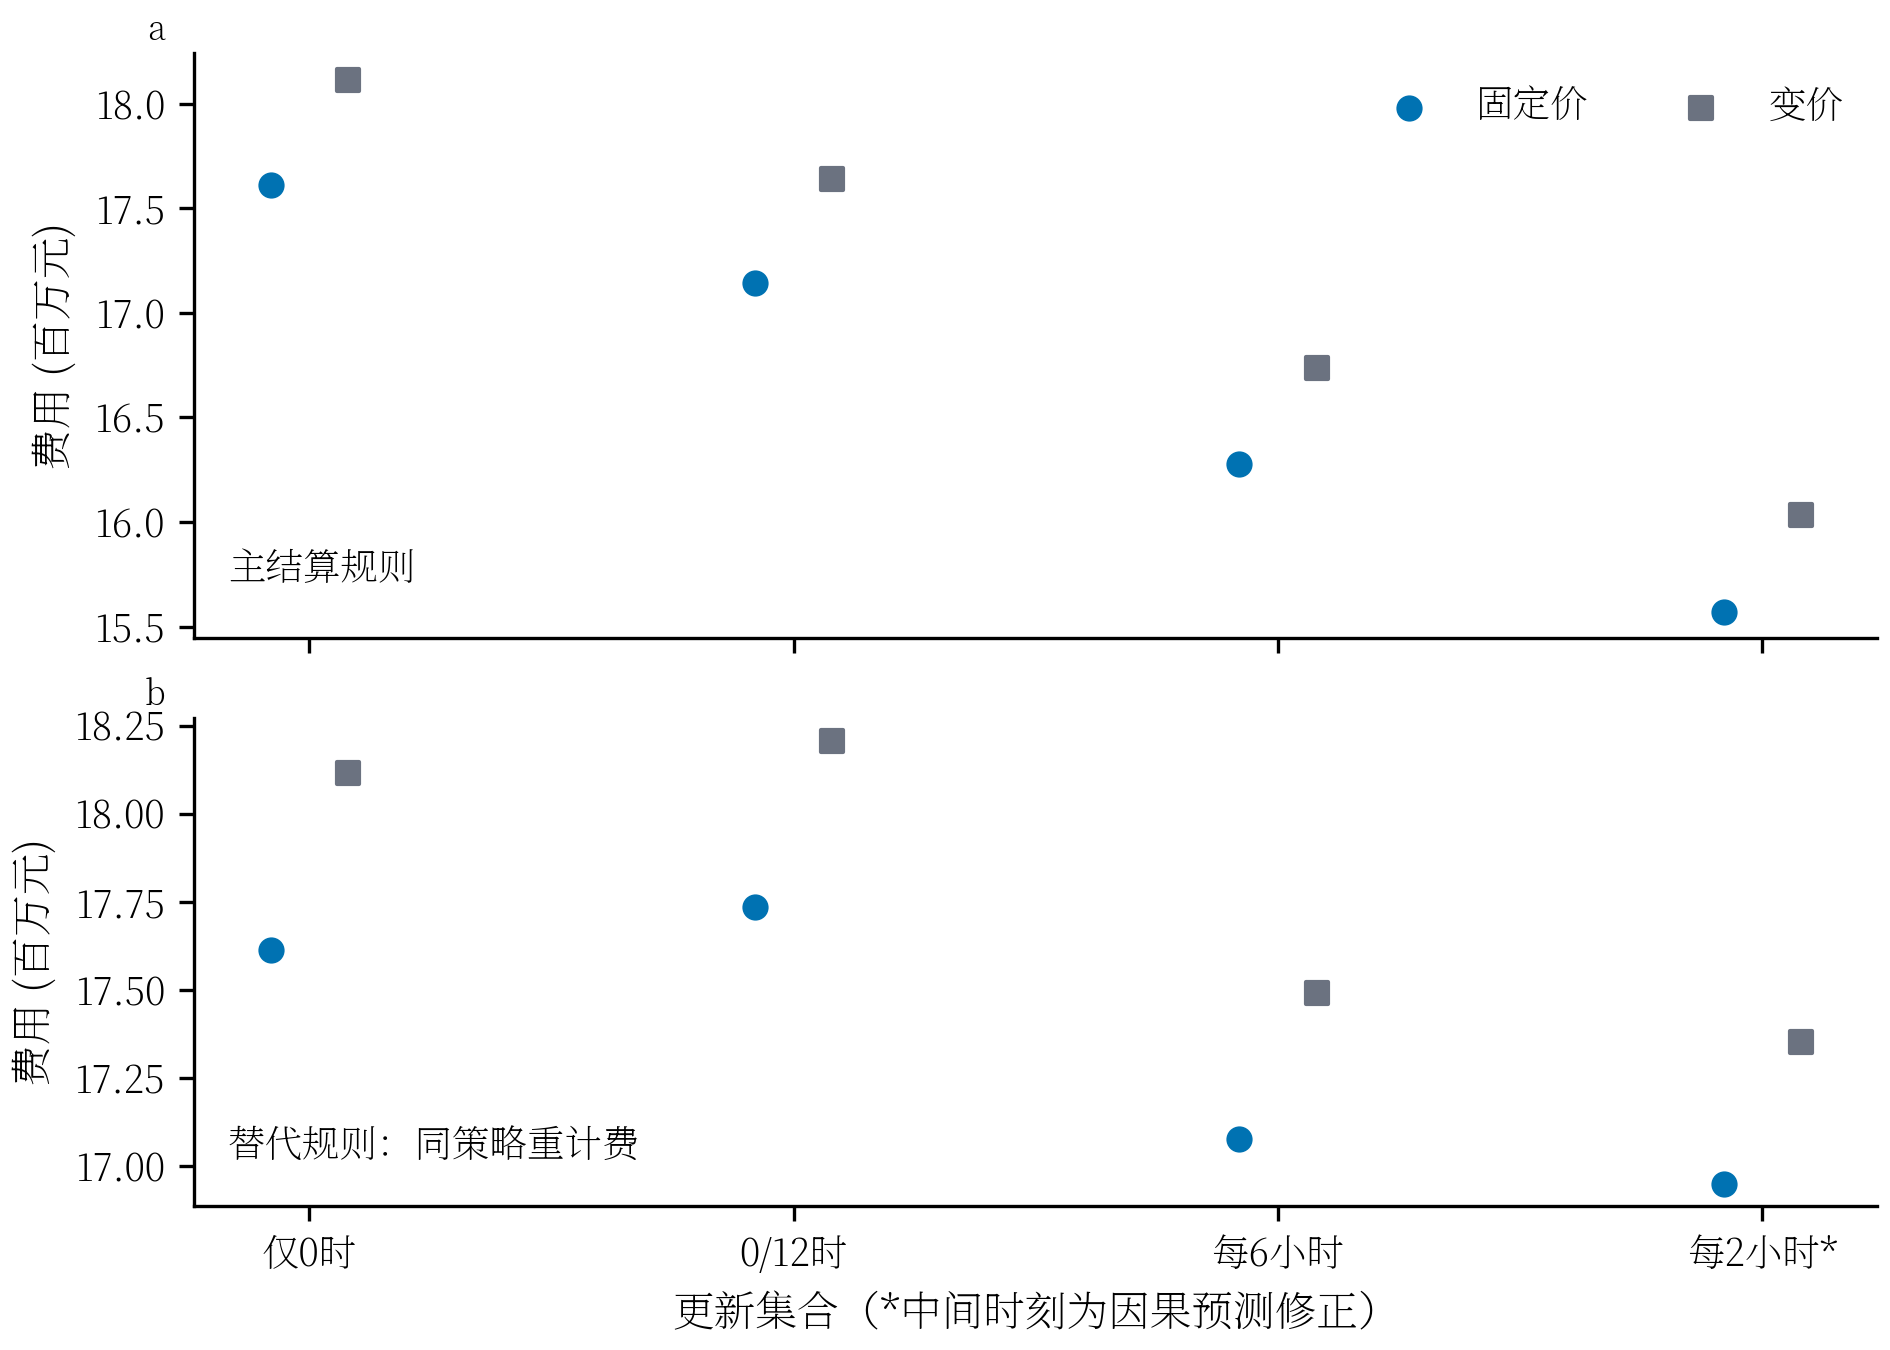
\includegraphics[width=0.96\textwidth]{figs/result_q3_update_frequency.png}
  \caption{固定与变动电价下不同更新集合的总费用，分别按主结算和替代结算重计。2小时方案使用因果合成更新。}
  \label{fig:q3-frequency}
\end{figure}
